\documentclass[12pt]{article}
\usepackage{hyperref}
\usepackage{amsmath, amssymb, amsfonts}
\usepackage[margin=1.2cm]{geometry}
\usepackage{xcolor}
\usepackage{graphicx}
\usepackage{enumitem}
\parindent 0pt
\newcommand{\lb}{\\$\left|\rightarrow\right.$}
\newcommand{\enter}{\\\textcolor{white}{1}}
\ExplSyntaxOn
\NewDocumentCommand{\bo}{m}
 {
   \bold_commas:n { #1 }
 }
\cs_new:Npn \bold_commas:n #1
 {
   \seq_set_split:Nnn \l_tmpa_seq { , } { #1 }
   \seq_map_indexed_function:NN \l_tmpa_seq \__bold_commas_aux:nn
 }
\cs_new:Npn \__bold_commas_aux:nn #1 #2
 {
   \textbf{#2}
   \int_compare:nNnTF { #1 } < { \seq_count:N \l_tmpa_seq }
     { , }
     { }
 }
\ExplSyntaxOff

\title{Wireless Communication (EX751 / EX715)\\[0.4em]\large Detailed PYQ}
\author{}
\date{\today}

\begin{document}
\maketitle
\vspace{5cm}
\textbf{Notes}
\begin{itemize}[noitemsep]
  \item PYQs from TU, IOE, BEX (EX751) and BEI (EX715) programmes combined, 2070--2082 BS. 22 papers: 16 BEX (2070--2080) and 6 BEI (2079--2082).
  \item BEX questions are in normal font; BEI questions are in \texttt{this monospace style}.
  \item Regular exam = \bo{bold}, Back exam = regular font. ``New Back (2066 \& Later Batch)'' counts as Back. Where a paper prints ``Regular / Back'' in one cell (\bo{76 Bh}, \bo{71 Bh}) it is taken as Regular.
  \item So: \bo{72 Ash} = BEX Regular, 73 Ma = BEX Back, \bo{\texttt{79 Bh}} = BEI Regular, \texttt{80 Ba} = BEI Back.
  \item Months: Ba = Baishakh, Bh = Bhadra, Ash = Ashwin, Ma = Magh, Ch = Chaitra.
  \item Keywords: (I) = Importance/Need/Significance, (+) = Advantage, (-) = Disadvantage, +Fig = Figure, +Eg = Example, Vs = Compare/Differentiate.
  \item Source defects are recorded as printed, not corrected: 2073 Magh Q2 asks for cluster size, cluster count and maximum users but prints \emph{no data}; the 2079 Chaitra header prints ``BEI'' on what is the EX751 (BEX) paper. Both are noted in place.
  \item Full verbatim transcriptions of all 22 papers: \texttt{ocr/EX-751\_EX-715\_OCR.md}.
\end{itemize}
\pagebreak
\tableofcontents
\pagebreak

%=======================================================================
\section{Introduction}
\begin{center}(2 Hours)\end{center}

  \subsection{Evolution of Wireless Communications (1G--5G)}
    \begin{enumerate}[topsep=0pt, noitemsep]
      \item Briefly explain evolution of wireless communications 1G--3G \hfill [6] (70 Ma, 72 Ma)
        \lb Evolution of wireless comm. in terms of technology \& worldwide market penetration \hfill [6] (70 Ma)
        \lb Evolution of cellular radio 1G--3G \hfill [4] (\bo{71 Bh})
        \lb Development of mobile comm., evolution path up to 3G technology \hfill [4] (74 Ma)
        \lb Evolution of different generations of cellular systems \hfill [4] (\bo{75 Bh})
        \lb Evolution from 1G to 2G, 2.5G in a TDMA-based cellular network \hfill [4] (71 Ma)
        \lb Evolution of wireless comm. from second to third generation \hfill [4] (\bo{73 Bh})
        \lb Evolution of wireless comm. from 1G to 4G, technology advancement \hfill [6] (\bo{76 Bh})
        \lb Features introduced from second to fifth generation of cellular systems \hfill [4] (\bo{78 Ch})
      \item Major benefits of wireless communication; brief description of the 4G wireless communication system \hfill [2+4] (\bo{\texttt{81 Bh}})
    \end{enumerate}

  \subsection{Comparison of Available Wireless Systems, Trends}
    \begin{enumerate}[topsep=0pt, noitemsep]
      \item 2G Vs 3G with +Eg of technologies used; prioritized handoff + cell dragging \hfill [4+2] (\bo{72 Ash})
      \item 3G Vs 4G mobile comm. standards, technology advancement \hfill [4] (\bo{75 Bh})
        \lb 1G Vs 2G Vs 3G Vs 4G standards, technology advancement \hfill [6] (\bo{74 Bh})
        \lb 3G Vs 4G \hfill [4] (\texttt{80 Ba, 81 Ba})
        \lb 2G Vs 3G Vs 4G standards, technology advancement \hfill [4] (\bo{\texttt{80 Bh}})
        \lb Improvements introduced in 2G, 3G and beyond-3G standards \hfill [6] (\bo{70 Bh})
        \lb Features of 4G other than 3G mobile communication system \hfill [5] (\bo{77 Ch})
    \end{enumerate}

  \subsection{Trends in Cellular Radio Beyond 3G}
    \begin{enumerate}[topsep=0pt, noitemsep]
      \item Basic trends in wireless communication beyond 3G, focusing on key technological changes \hfill [4] (\bo{\texttt{82 Bh}})
      \item Forward \& reverse channel; 5G Vs 4G mobile communication \hfill [2+2] (\bo{\texttt{79 Bh}}, \bo{79 Ch})
        \lb Define forward and reverse channel \hfill [2] (\bo{\texttt{80 Bh}})
        \lb Forward \& reverse channel; list the features of 5G \hfill [2+2] (\bo{80 Ch})
    \end{enumerate}

\pagebreak
%=======================================================================
\section{Cellular Mobile Communication Concepts}
\begin{center}(4 Hours)\end{center}

  \subsection{Frequency Reuse and Channel Assignment}
    \begin{enumerate}[topsep=0pt, noitemsep]
      \item Frequency reuse concept; co-channel reuse ratio in detail \hfill [6] (72 Ma)
        \lb Minimizing reuse distance maximizes spectral efficiency (I) \hfill [4] (\bo{74 Bh})
        \lb Cellular concept for $N = 7$ \hfill [3] (\bo{76 Bh})
      \item Prove co-channel reuse ratio $Q = \sqrt{3N}$, $N = i^2 + ij + j^2$; find optimal $N$ for
        omni-directional, 120° and 60° sectoring, SIR = 15 dB worst case, path loss exponent
        $n = 4$, considering trunking efficiency
        \enter\hfill [4+4] (\bo{71 Bh})
        \lb Prove $Q = \sqrt{3N}$; find optimal $N$ for omni, ``1200'' (120°) and 60° sectoring,
        SIR = 15 dB, $n = 3$; comment on results \hfill [3+5] (\bo{\texttt{79 Bh}})
        \lb Derive the formula for co-channel reuse ratio $Q = \sqrt{3N}$ \hfill [4] (\bo{\texttt{80 Bh}})
        \lb Co-channel Vs adjacent channel interference; prove $Q = \sqrt{3N}$;
        20 MHz total duplex spectrum, 25 kHz per simplex channel --- find
        (a) number of duplex channels, (b) channels per cell for $N = 4$
        \enter\hfill [3+4+3] (\bo{70 Bh})
        \lb Co-channel Vs adjacent channel interference; prove $Q = \sqrt{3N}$ \hfill [3+3] (\bo{\texttt{81 Bh}})
        \lb Obtain $S/I = \sqrt[n]{3N}/i_0$ \hfill [4] (74 Ma)
      \item For a seven-cell reuse pattern, find minimum distance between centres of
        co-channel cells; area of each cell is uniform and equal to 23 km² \hfill [4] (\bo{74 Bh})
    \end{enumerate}

  \subsection{Handoff Strategies, Types, Priorities, Practical Considerations}
    \begin{enumerate}[topsep=0pt, noitemsep]
      \item Define handoff margin +Fig \hfill [3] (\bo{75 Bh})
      \item What is hand off? Handoff strategy used in GSM \hfill [8] (70 Ma)
      \item Handover process in cellular system; types of handover with application \hfill [6] (74 Ma)
        \lb Handover process; various practical handover considerations \hfill [4+4] (\bo{78 Ch})
        \lb Practical handoff considerations \hfill [4] (\texttt{79 Bh}, 73 Ma)
        \lb Prioritized handoff; cell dragging \hfill [2] (\bo{72 Ash})
        \lb Cell dragging; how hand off is processed in a cellular system \hfill [2+4] (\bo{73 Bh})
        \lb Improper handoff situation Vs proper handoff situation \hfill [4] (\bo{76 Bh})
        \lb What is Hand-off? Proper and improper HO with necessary drawing \hfill [1+3] (\texttt{81 Ba})
      \item Two schemes for prioritizing handoff; define grade of service, traffic intensity,
        average holding time and block call \hfill [3+4] (\bo{\texttt{82 Bh}})
    \end{enumerate}

  \subsection{Interference and System Capacity}
    \begin{enumerate}[topsep=0pt, noitemsep]
      \item Explain the terminologies (i) co-channel interference (ii) adjacent interference \hfill [2.5+2.5] (\bo{80 Ch})
      \item What is cell footprint? Explain interference tier in brief \hfill [1+4] (\bo{80 Ch})
      \item Interference in wireless/mobile communication \hfill [4] (\texttt{80 Ba, 81 Ba})
    \end{enumerate}

  \subsection{Grade of Service (GoS) and Trunking}
    \begin{enumerate}[topsep=0pt, noitemsep]
      \item GoS, and how it is measured in a ``blocked call cleared'' trunking system;
        cellular provider uses digital TDMA tolerating SIR = 15 dB worst case,
        path loss exponent $n = 3$ --- find optimal $N$ for
        (a) omni-directional antennas, (b) 120° sectoring, (c) 60° sectoring; comment
        \enter\hfill [3+5] (\bo{\texttt{79 Bh}})
      \item Urban area, population two million; System A has 394 cells with 19 channels each.
        Find the number of users supported at 2\% blocking if each user averages two calls per
        hour at an average call duration of three minutes. Assuming trunk systems operate at
        maximum capacity, compute the percentage market penetration of the cellular provider
        \enter\hfill [5] (\texttt{80 Ba, 81 Ba}, \bo{79 Ch})
      \item Mobile radio system: each user averages three calls per hour, each call lasting
        an average of 5 minutes. (a) traffic intensity per user; (b) number of users at 1\%
        blocking with only one channel; (c) number of users at 1\% blocking with five trunked
        channels; (d) if the users found in (c) are suddenly doubled, the new blocking
        probability of the five-channel trunked system --- justify whether performance is acceptable
        \enter\hfill [2+2+2+3] (\bo{77 Ch})
        \enter Traffic (A) in erlangs for B\%:
        \begin{center}\small
        \begin{tabular}{|c|c|c|c|c|c|c|c|c|}
        \hline
        Trunks $N$ & 0.1\% & 0.2\% & 0.5\% & 1\% & 1.2\% & 3\% & 5\% & 7\% \\ \hline
        1 & 0.001 & 0.002 & 0.005 & 0.010 & 0.012 & 0.031 & 0.053 & 0.075 \\ \hline
        2 & 0.046 & 0.065 & 0.105 & 0.153 & 0.168 & 0.282 & 0.381 & 0.470 \\ \hline
        3 & 0.194 & 0.249 & 0.349 & 0.455 & 0.489 & 0.715 & 0.899 & 1.06 \\ \hline
        4 & 0.439 & 0.535 & 0.701 & 0.869 & 0.922 & 1.26 & 1.52 & 1.75 \\ \hline
        5 & 0.762 & 0.900 & 1.13 & 1.36 & 1.43 & 1.88 & 2.22 & 2.50 \\ \hline
        \end{tabular}
        \end{center}
      \item Cluster $N = 7$, blocking probability 1\%, average call length two minutes,
        average request rate 1 call/hour per user --- find the traffic capacity loss for a
        blocked-calls-cleared system due to trunking for 57 channels when going from
        omnidirectional antennas to 60° sectored antennas
        \enter\hfill [2+2+2] (\texttt{81 Ba})
        \enter GOS / Channel table as printed:
        \begin{center}\small
        \begin{tabular}{|c|c|c|c|}
        \hline
        GOS / Channel & 0.5\% & 1\% & 2\% \\ \hline
        1  & .005  & .0101 & .0204 \\ \hline
        9  & 3.333 & 3.783 & 4.345 \\ \hline
        19 & 10.33 & 11.23 & 12.33 \\ \hline
        54 & 39.47 & 41.51 & 44.00 \\ \hline
        57 & 42.1  & 44.2  & 46.8  \\ \hline
        \end{tabular}
        \end{center}
      \item City of 1500 km² covered by a 12-cell system, each cell radius 1.387 km, total
        spectrum 28.5 MHz, full duplex channel bandwidth 25 MHz, GOS 0.02 for a
        blocked-calls-cleared system, offered traffic per user 0.03 Erlangs, traffic intensity
        per cell 84 Erlang --- compute (a) number of cells in the service area, (b) channels
        per cell, (c) maximum carrier traffic, (d) total users served at 2\% GOS,
        (e) mobiles per unique channel, (f) theoretical maximum users served at one time
        \enter\hfill [12] (72 Ma)
      \item Cellular system with 32 cells, each of 1.6 km radius, reuse factor 7, supporting
        336 traffic channels in total --- determine the total geographical area covered, the
        number of traffic channels per cell and the total number of simultaneous calls supported
        \enter\hfill [4] (\bo{\texttt{82 Bh}})
      \item Determine (a) the cell cluster size, (b) the number of cell clusters in the
        service area, (c) the maximum number of users in the service area at any instant
        \hfill [6] (73 Ma)
        \enter\emph{The paper prints no data for this question --- recorded as printed.}
    \end{enumerate}

  \subsection{Coverage and Capacity Enhancement}
    \begin{enumerate}[topsep=0pt, noitemsep]
      \item Why do we need the microcell zone concept? Explain it in brief \hfill [3] (\texttt{80 Ba, 81 Ba}) [1+3] (\bo{79 Ch})
      \item Telephone network company expanding capacity in a city: sectoring Vs cell splitting
        --- as a cellular planning engineer, which option is best and why? \hfill [5] (\bo{75 Bh}) [4] (\bo{\texttt{81 Bh}})
        \lb How cell splitting and sectoring improve coverage and capacity \hfill [5] (\bo{73 Bh})
      \item Techniques used for enhancing capacity \& coverage in a cellular radio network \hfill [8] (71 Ma)
    \end{enumerate}

\pagebreak
%=======================================================================
\section{Radio Wave Propagation in Mobile Network Environment}
\begin{center}(12 Hours)\end{center}

  \subsection{Free Space Propagation, Radiated Power and Electric Field}
    \begin{enumerate}[topsep=0pt, noitemsep]
      \item Free space propagation: receiver 10 km from a 50 W transmitter, carrier 900 MHz,
        $G_T{=}1$, $G_R{=}2$, receiver antenna purely real 50\,$\Omega$ and matched --- find
        (i) power received, (ii) magnitude of E-field at the receiver antenna,
        (iii) power flux density, (iv) rms voltage applied to the receiver input
        \enter\hfill [8] (\texttt{80 Ba, 81 Ba}) [2+2+2+2] (\bo{78 Ch})
      \item TX output 165 W at 325 MHz into a 12 dBi antenna; RX 15 km away with 6 dBi gain;
        find power delivered to the receiver (free-space, no other losses or mismatches)
        \enter\hfill [6] (\bo{\texttt{80 Bh}})
      \item Link budget: BS transmitter 10 W at 250 MHz, 20 m of RF coax at 3 dB/100 m,
        antenna gain 9 dBi; receiving antenna 25 km away, gain 4 dBi; negligible feeder loss
        but 0.2 dB receiver mismatch loss (50\,$\Omega$ system) --- find power delivered to the
        receiver assuming free-space propagation
        \enter\hfill [8] (\bo{72 Ash})
      \item Determine the radio coverage range of a base station transmitting 150 W,
        receiver threshold $-104$ dBm, path loss at the first metre 15 dB,
        path loss exponent 4 \hfill [6] (\bo{70 Bh})
      \item Mobile 5 km from a base station with a vertical $\lambda/4$ monopole of gain 2.55 dB;
        E-field at 1 km from the transmitter is $10^{-3}$ V/m, carrier 900 MHz ---
        (a) length and effective aperture of the receiving antenna; (b) received power using the
        two-ray ground reflection model, TX height 50 m, RX height 1.5 m
        \enter\hfill [6] (\bo{71 Bh})
      \item Cordless phone operating at 52000 kHz with a range of 50 m ---
        determine the free space path loss \hfill [6] (\bo{77 Ch}) [2+4] (\bo{80 Ch})
      \item Transmitter produces 50 W --- express transmit power in (i) dBm and (ii) dBW;
        with 50 W into a unity-gain antenna at 900 MHz find the received power in dBm at a
        free-space distance of 100 m, and $P_r$(10 km), assuming unity receive gain
        \enter\hfill [1+1+2+2] (\texttt{81 Ba})
      \item Explain basic propagation models; compute the far-field distance for an antenna of
        maximum dimension 1 m operating at 900 MHz \hfill [3+3] (\bo{79 Ch})
    \end{enumerate}

  \subsection{Large-Scale Path Loss: Propagation Mechanisms}
    \begin{enumerate}[topsep=0pt, noitemsep]
      \item Large scale Vs small scale propagation model; propagation mechanisms
        which have impact on propagation in a mobile environment \hfill [3+6] (\bo{72 Ash})
        \lb The three basic radio wave propagation mechanisms \hfill [3] (\bo{73 Bh})
        \lb Mobile radio propagation in terms of large scale path loss and small scale fading \hfill [8] (72 Ma)
      \item Define path loss; parameters of a mobile multipath channel used to classify the
        various types of fading \hfill [2+4] (\bo{\texttt{80 Bh}})
      \item Derive the expression for phase difference in the two-ray free space
        propagation model \hfill [8] (\bo{71 Bh})
        \lb Derive path difference and phase difference between the LOS path and the
        ground-reflected (GR) path in the two-ray model using simple geometrical relations \hfill [6] (\bo{\texttt{81 Bh}})
        \lb Diffraction in radio wave propagation; derive an expression for phase difference
        in the Fresnel Zone Geometry model \hfill [2+6] (\bo{\texttt{79 Bh}})
        \lb (+) of the two-ray propagation model over the free space path loss model;
        derive the path loss equation for the two-ray model +Fig \hfill [2+6] (\bo{76 Bh})
      \item What is known as scattering? Derive an expression for the two-ray ground
        reflected model \hfill [2+8] (\bo{74 Bh})
      \item Path loss Vs fading of signal; time dispersion fading and its types \hfill [2+6] (\bo{71 Bh})
    \end{enumerate}

  \subsection{Practical Link Budget Design Using Path Loss Models}
    \begin{enumerate}[topsep=0pt, noitemsep]
      \item Explain the log-distance path loss model \hfill [4] (\bo{77 Ch})
      \item Estimate the distance to be maintained on the reverse link between one BTS and a
        mobile, with an appropriate link budget diagram:
        (i) mobile antenna 20 dBi, TX power 15 dBm, receive sensitivity $-75$ dBm;
        (ii) BTS antenna 5 dBi, TX power 20 dBm, receive sensitivity $-80$ dBm;
        (iii) short cables, 3 dB loss each side, 900 MHz.
        Use Okumura's model for mean path loss with $G(\text{Area}) = 9$ dB, $A_{mu} = 43$ dB,
        $h_{re} = 10$ m, $h_{te} = 100$ m; link margin (reverse link) = 10 dB
        \enter\hfill [10] (\bo{76 Bh})
      \item Estimate the feasibility of a 10 km wireless link in a suburban area with one access
        point and one client radio, using the Okumura model for path loss; median attenuation
        20 dB, gain due to environment 13 dB, AP antenna height 100 m, client antenna height 10 m:
        (a) AP antenna 5 dBi, TX 20 dBm, sensitivity $-80$ dBm;
        (b) client antenna 20 dBi, TX 15 dBm, sensitivity $-75$ dBm;
        (c) short cables, 3 dB loss each side, 2.4 GHz
        \enter\hfill [12] (\bo{74 Bh})
    \end{enumerate}

  \subsection{Outdoor Propagation Models}
    \begin{enumerate}[topsep=0pt, noitemsep]
      \item Explain any two outdoor propagation models used in the mobile radio environment
        \hfill [3+3] (\bo{75 Bh}, 71 Ma) [5] (73 Ma)
      \item Necessary conditions for the Okumara and Hata models \hfill [2+2] (\bo{80 Ch}, \bo{79 Ch})
        \lb Compare the Okumura model with the Hata model \hfill [4] (\bo{\texttt{81 Bh}})
      \item Okumura model: median path loss for T--R separation 50 km, transmit antenna
        effective height 100 m, receive antenna effective height 10 m, suburban area,
        correction factor 9 dB at 900 MHz, median attenuation relative to free space 43 dB
        \enter\hfill [4+4] (74 Ma)
        \lb Okumura model, suburban, $d{=}50$ km, $h_{te}{=}100$ m, $h_{re}{=}10$ m, BS radiating
        EIRP of 1 kW at 900 MHz --- find EIRP (dBm) and the power at the receiver where the
        receiving antenna gain is 10 dB, medium attenuation factor 43 dB, gain due to area 9 dB
        \enter\hfill [4+2+2] (\bo{\texttt{80 Bh}}) [5] (\bo{\texttt{82 Bh}})
        \lb Okumura model: compute the transmitter--receiver separation if median loss is
        167 dB at carrier 2.1 GHz, transmitting antenna 40 m, receiving antenna 2 m,
        large city, $A_{mu} = 34$ dB, $G_{area} = 0$ dB \hfill [8] (\bo{77 Ch})
      \item Hata model: correction factor and pathloss for a medium-size city, $f_c{=}950$ MHz,
        BS antenna 45 m, distance 10 km, MS antenna 5 m; compute free space pathloss and
        compare with Hata pathloss \hfill [4+4] (\bo{\texttt{79 Bh}})
        \lb Hata model: maximum cell radius and corresponding cell area, BS transmitting 50 W,
        minimum acceptable received power at MS $-91$ dBm, carrier 900 MHz,
        $h_{BS}{=}30$ m, $h_{MS}{=}1$ m, medium sized city \hfill [6] (73 Ma)
        \lb Hata model: propagation path loss for a 900 MHz cellular system in a large urban
        city, BS transmitter antenna 100 m, mobile receiver antenna 2 m, mobile at 4 km
        \hfill [7] (\bo{73 Bh})
        \enter Hints printed on the 73 Bh paper:\\
        \mbox{}\hfill {\small $L_{50} = 69.55 + 26.16\log f_c - 13.82\log h_t - \alpha(h_r) + (44.9 - 6.55\log h_t)\log d$}\hfill\mbox{}\\
        \mbox{}\hfill {\small $\alpha(h_r) = (1.1\log f_c - 0.7)h_r - (1.56\log f_c - 0.8)$ \quad small to medium city}\hfill\mbox{}\\
        \mbox{}\hfill {\small $\alpha(h_r) = 8.29(\log 1.54 h_r)^2 - 1.1$ \quad large city, $f_c \le 300$ MHz}\hfill\mbox{}\\
        \mbox{}\hfill {\small $\alpha(h_r) = 3.2(\log 11.75 h_r)^2 - 4.97$ \quad large city, $f_c > 300$ MHz}\hfill\mbox{}
      \item Two-ray mobile point-to-point propagation model: path loss at 800 MHz,
        transmitting antenna 30 m, receiving antenna 2 m, distance 10 km;
        compare with the free-space path loss model \hfill [4+4] (70 Ma)
      \item What do you mean by the Ericsson Multiple Breakpoint model? \hfill [2] (\bo{\texttt{80 Bh}})
    \end{enumerate}

  \subsection{Indoor Propagation Models}
    \begin{enumerate}[topsep=0pt, noitemsep]
      \item Explain indoor propagation models (any two) \hfill [8] (\bo{70 Bh})
      \item Factors that influence the indoor propagation model \hfill [5] (\bo{\texttt{82 Bh}})
    \end{enumerate}

  \subsection{Small Scale Fading, Multipath Parameters, Doppler}
    \begin{enumerate}[topsep=0pt, noitemsep]
      \item What is small scale fading? Types in radio propagation + factors which influence it
        \hfill [2+4+4] (\bo{75 Bh}) [4+4] (\texttt{80 Ba, 81 Ba}) [2+2] (73 Ma) [3+6] (72 Ma)
        \lb Fading; factors influencing small-scale fading; derive the relation for Doppler's shift
        \hfill [1+2+5] (\bo{78 Ch})
        \lb Define fading; its different types based on delay spread and Doppler spread \hfill [1+3] (\texttt{81 Ba})
      \item Parameters of the mobile multipath channel \hfill [7] (71 Ma)
      \item Define Doppler spread; derive the expression for Doppler shift \hfill [2+4] (\texttt{81 Ba})
        \lb Significance of frequency dispersion in wireless communication;
        derive the relation for Doppler spread \hfill [2+4] (\bo{\texttt{82 Bh}})
        \lb Doppler's effect in small scale fading \hfill [2] (\bo{80 Ch})
      \item Doppler spread; types of small-scale fading based on Doppler spread; mean excess
        delay and rms delay spread for the multipath profile below; 90\% and 50\%
        coherence bandwidth of the channel \hfill [4+4] (70 Ma)
        \begin{center}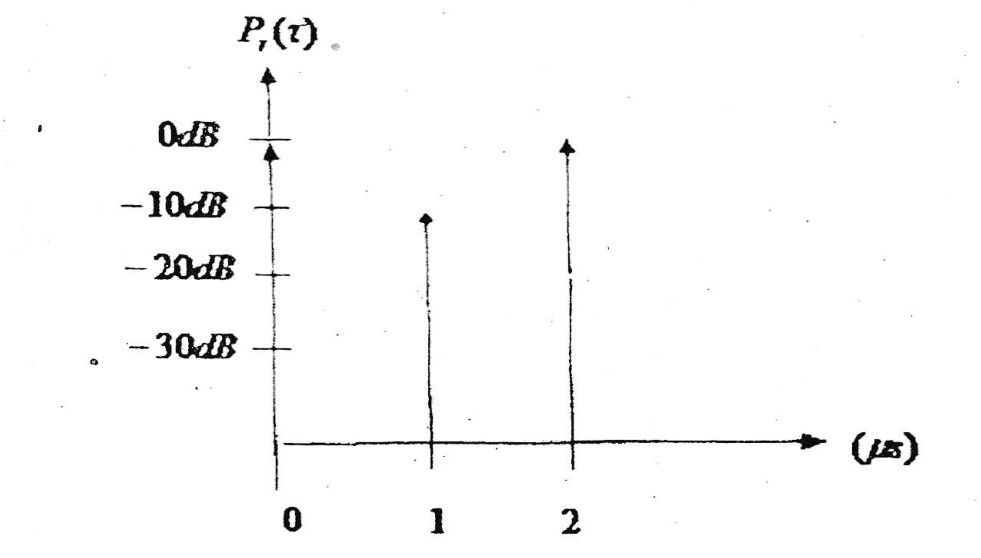
\includegraphics[width=3.2in]{images/wl_70ma_pdp.png}\end{center}
      \item Coherence bandwidth and coherence time --- definitions and significance in
        mobile radio propagation \hfill [4] (73 Ma, \bo{77 Ch}) [2+5] (\bo{\texttt{82 Bh}})
        \lb Doppler spread and coherence bandwidth; classify fading on the basis of
        rms delay spread and coherence time \hfill [4+4] (74 Ma)
        \lb Frequency selective fading; relationship between coherence bandwidth and
        delay spread in the time domain \hfill [2+7] (\bo{79 Ch})
      \item Determine the smallest symbol period $T_s$, and thus the greatest symbol rate,
        that can be sent through an RF channel with the power delay profile below without
        using an equalizer; modulation gives suitable BER whenever
        $\sigma_\tau / T_s \le 0.1$ \hfill [8] (\bo{75 Bh})
        \begin{center}\small
        \begin{tabular}{|l|c|c|c|c|}
        \hline
        Power [dB]  & 0 & 0  & $-10$ & $-20$ \\ \hline
        Delay [µs]  & 0 & 50 & 75    & 100   \\ \hline
        \end{tabular}
        \end{center}
      \item Mean excess delay, rms delay spread and maximum excess delay for the multipath
        profile $P_r(\tau) = (-20\,\text{dB}, -10\,\text{dB}, -10\,\text{dB}, 0\,\text{dB})$ at
        $\tau = (0, 1, 2, 5)$ second; also estimate the 50\% coherence bandwidth
        \enter\hfill [6] (\bo{\texttt{81 Bh}})
      \item rms delay spread and 90\% coherence bandwidth of the channel below; is the channel
        flat fading or frequency selective for (i) an AMPS system of transmission bandwidth
        30 kHz, (ii) a GSM system of transmission bandwidth 200 kHz? \hfill [6] (71 Ma)
        \begin{center}\small
        \begin{tabular}{|l|c|c|c|c|}
        \hline
        Power [dB]  & 0 & $-10$ & $-20$ & $-23$ \\ \hline
        Delays [ns] & 0 & 100   & 200   & 400   \\ \hline
        \end{tabular}
        \end{center}
    \end{enumerate}

  \subsection{Types of Small-Scale Fading; Rayleigh and Ricean Distribution}
    \begin{enumerate}[topsep=0pt, noitemsep]
      \item Rayleigh fading channel Vs Rician fading channel, with appropriate expressions \hfill [2] (71 Ma)
        \lb Rayleigh and Ricean fading distribution \hfill [5] (70 Ma, \bo{72 Ash}) [5] (\bo{73 Bh})
      \item What is frequency selective fading? Explain the Rayleigh distribution in brief \hfill [2+4] (\bo{80 Ch})
    \end{enumerate}

\pagebreak
%=======================================================================
\section{Modulation--Demodulation Methods in Mobile Communications}
\begin{center}(4 Hours)\end{center}

  \subsection{Digital Linear Modulation: BPSK, DPSK, QPSKs}
    \begin{enumerate}[topsep=0pt, noitemsep]
      \item QPSK: transmission \& detection process \hfill [6] (\bo{75 Bh}) [8] (72 Ma)
        \lb QPSK transmission \& detection +Fig, constellation diagram \hfill [8] (\bo{\texttt{81 Bh}})
        \lb QPSK modulation with its appropriate equation and constellation diagram \hfill [7] (\bo{73 Bh})
      \item OQPSK transmitter \& receiver; why $\pi/4$-QPSK is preferred over OQPSK \hfill [5+2] (\bo{71 Bh})
      \item DPSK modulation: transmitter and receiver; pseudo-noise (PN) sequence and why it is used
        \hfill [4+2+2] (72 Ma)
      \item BPSK against QPSK modulation \hfill [5] (73 Ma)
    \end{enumerate}

  \subsection{Constant Envelope Modulation: MSK, GMSK}
    \begin{enumerate}[topsep=0pt, noitemsep]
      \item MSK as a special type of continuous-phase FSK and OQPSK;
        compare OQPSK, MSK and GMSK in bandwidth efficiency and power efficiency;
        which is suitable for GSM modulation and why \hfill [3+3+2] (\texttt{80 Ba, 81 Ba})
        \lb What is MSK modulation? \hfill [2] (\bo{80 Ch})
        \lb MSK and GMSK modulation techniques \hfill [4] (\bo{76 Bh})
      \item Advantages of digital modulation over analog; GMSK transmission \& detection
        process with block diagram and constellation diagram \hfill [2+6] (\bo{\texttt{79 Bh}}) [8] (\texttt{81 Ba})
      \item MSK \& GMSK modulation techniques; OFDM modulator and demodulator +Fig \hfill [8] (70 Ma)
    \end{enumerate}

  \subsection{M-ary Modulation (MPSK, MFSK, QAM) and OFDM}
    \begin{enumerate}[topsep=0pt, noitemsep]
      \item OFDM operation +Fig (block diagram of transmitter \& receiver)
        \hfill [8] (\bo{74 Bh}, \bo{\texttt{80 Bh}}, \bo{78 Ch})
        \lb OFDM: generalize the modulation and demodulation technique \hfill [8] (71 Ma)
        \lb OFDM principle; different types of spread spectrum modulation techniques \hfill [4+4] (\bo{70 Bh})
        \lb OFDM transmitter in brief \hfill [4] (\bo{79 Ch})
        \lb OFDM receiver in brief \hfill [4] (\bo{80 Ch})
        \lb OFDM transmitting side block diagram; (+) and (-) \hfill [4+4] (\bo{\texttt{82 Bh}})
      \item Why do we need M-ary QAM? Compare 16-QAM and 16-PSK using their
        constellation diagrams \hfill [2+6] (\bo{77 Ch})
    \end{enumerate}

  \subsection{Spread Spectrum: PN Sequences, DS and FH}
    \begin{enumerate}[topsep=0pt, noitemsep]
      \item Direct Sequence \& Frequency Hopped Spread Spectrum techniques \hfill [4] (73 Ma)
        \lb Define spread spectrum modulation; DSSS with block diagrams of transmitter
        and receiver \hfill [2+6] (\bo{\texttt{82 Bh}}) [6] (\texttt{81 Ba}) [2+5] (\bo{80 Ch})
        \lb Define spread spectrum; FHSS with relevant diagram \hfill [2+5] (\bo{79 Ch})
        \lb FHSS operation with a neat block diagram \hfill [4] (\bo{73 Bh})
      \item Advantages of spread spectrum modulation technique in wireless communication \hfill [4] (\bo{76 Bh})
        \lb Major disadvantages of the spread spectrum system \hfill [2] (\bo{77 Ch})
    \end{enumerate}

\pagebreak
%=======================================================================
\section{Equalization and Diversity Techniques}
\begin{center}(4 Hours)\end{center}

  \subsection{Equalization: Linear, Non-linear, Adaptive}
    \begin{enumerate}[topsep=0pt, noitemsep]
      \item Equalization (I) in wireless communication; describe the signal processing operation
        that minimizes the effects of ISI \hfill [2+6] (\bo{75 Bh}) [2+5] (72 Ma) [4] (73 Ma)
        \lb Signal processing operation that minimizes ISI; RACK receiver; structure of the
        linear transversal equalizer +Fig \hfill [2+1+4] (\bo{\texttt{82 Bh}})
      \item Training and tracking modes of operation for adaptive equalizers \hfill [4] (\bo{78 Ch})
        \lb Why equalization is needed; training and tracking modes in detail \hfill [1+3] (\bo{73 Bh})
      \item MSE algorithm: determine the optimal solution of the weights, with appropriate
        diagram and derivation \hfill [8] (\bo{\texttt{79 Bh}}) [7] (\bo{80 Ch}, \bo{79 Ch})
      \item Maximum Likelihood Sequence Estimation (MLSE) +Fig;
        define time diversity and explain two implementations of it \hfill [6+1+5] (\bo{72 Ash})
        \lb MLSE equalization +Fig \hfill [4] (71 Ma, 72 Ma)
        \lb Working of MLSE \hfill [4] (\bo{\texttt{81 Bh}})
      \item Adaptive equalization algorithms (any two) \hfill [4] (73 Ma)
        \lb Adaptive Equalization \hfill [5] (74 Ma)
      \item Interleaving: working principle +Fig \hfill [4] (\bo{\texttt{81 Bh}})
        \lb Why interleaving is needed in wireless communication; its working in brief \hfill [4] (\bo{\texttt{80 Bh}})
        \lb Define interleaving; how equalization offsets the ISI introduced by the multipath
        time-dispersive channel, using an adaptive equalizer as example \hfill [2+6] (\texttt{81 Ba})
    \end{enumerate}

  \subsection{Diversity Methods and Combining}
    \begin{enumerate}[topsep=0pt, noitemsep]
      \item Why equalization \& diversity are needed in wireless communication systems;
        diversity reception methods used for space diversity; explain any one \hfill [3+3+2] (\texttt{80 Ba, 81 Ba})
      \item Why is there a need to implement diversity? Maximum ratio combining
        space diversity technique \hfill [2+2] (\bo{\texttt{80 Bh}})
        \lb Diversity (I) in wireless communication; different types of diversity techniques \hfill [2+6] (\bo{71 Bh})
        \lb Diversity techniques; combining methods used for space diversity \hfill [4+4] (74 Ma)
        \lb Why implement diversity? Various diversity combining techniques \hfill [4+6] (\bo{74 Bh})
        \lb Various space diversity techniques along with block diagrams \hfill [4] (73 Ma)
        \lb What is diversity? Any two types of diversity techniques in detail \hfill [2+6] (\bo{70 Bh})
        \lb How diversity improves the quality of the network \hfill [2] (\bo{76 Bh})
      \item Discuss and compare different types of antenna diversity technique \hfill [4] (71 Ma)
        \lb Feedback Vs maximum ratio combining technique used in antenna diversity \hfill [4] (\bo{78 Ch})
    \end{enumerate}

  \subsection{RAKE Receivers and Interleaving}
    \begin{enumerate}[topsep=0pt, noitemsep]
      \item RACK (RAKE) receiver: working of an M-branch receiver \hfill [8] (\bo{72 Ash}) [3+5] (\bo{77 Ch})
        \lb RAKE receiver: operation with appropriate block diagram \hfill [4] (70 Ma, \bo{76 Bh})
        \lb What is a RAKE receiver and how does it exploit the concept of time diversity? \hfill [3] (\bo{73 Bh})
        \lb RAKE receiver \hfill [4] (\texttt{79 Bh})
    \end{enumerate}

\pagebreak
%=======================================================================
\section{Speech and Channel Coding Fundamentals}
\begin{center}(4 Hours)\end{center}

  \subsection{Speech Characteristics, Frequency Domain Coding, Vocoders}
    \begin{enumerate}[topsep=0pt, noitemsep]
      \item Characteristics of the speech signal
        \hfill [8] (\bo{72 Ash}) [6] (\bo{77 Ch}) [3] (73 Ma, \texttt{79 Bh}) [3] (\bo{80 Ch})
        \lb Characteristics of speech signals; how they are used in designing coders \hfill [8] (\bo{72 Ash}) [4] (\bo{\texttt{82 Bh}}, \texttt{81 Ba})
      \item Vocoder (I); explain any two predictive coders \hfill [2+6] (\bo{70 Bh})
        \lb Vocoders with block diagram; different kinds of vocoders \hfill [2+3] (73 Ma) [3+5] (\bo{\texttt{81 Bh}})
        \lb Operation of a vocoder with the help of a block diagram \hfill [4] (\bo{73 Bh}) [6] (\texttt{81 Ba})
        \lb Formant vocoder operation; characteristics of the speech signal \hfill [4+4] (\bo{71 Bh})
        \lb Why we need speech coding techniques; basic concept of VOCODER \hfill [4+4] (70 Ma) [2+6] (\bo{78 Ch})
        \lb Waveform and voice coding techniques; characteristics of speech;
        GSM CODEC +Fig \hfill [4+2+2] (74 Ma)
        \lb Operation of any two source coders used in speech coding \hfill [6] (\bo{74 Bh})
        \lb Types of frequency domain coding of speech \hfill [4] (\bo{73 Bh})
      \item Characteristics of the speech signal; Linear Predictive Coder (LPC)
        with neat block diagram \hfill [2+6] (\texttt{80 Ba, 81 Ba}, 72 Ma) [3+5] (\bo{\texttt{79 Bh}}, 73 Ma, \bo{76 Bh}) [2+6] (\bo{75 Bh}, 72 Ma)
        \lb Types of linear predictive coder \hfill [6] (71 Ma)
      \item Sub-band coding with transmitter and receiver \hfill [6] (\bo{\texttt{80 Bh}})
    \end{enumerate}

  \subsection{Channel Coding: Block, Convolutional, Turbo}
    \begin{enumerate}[topsep=0pt, noitemsep]
      \item What is channel coding? \hfill [2] (71 Ma)
      \item 7-bit Hamming code method with a relevant example \hfill [5] (\bo{80 Ch})
      \item Convolutional encoding and decoding \hfill [5] (\bo{74 Bh})
      \item Viterbi decoding algorithm \hfill [3] (\bo{75 Bh}, 70 Ma, \bo{72 Ash}) [5] (\bo{73 Bh})
      \item Define turbo coding \hfill [2] (\bo{\texttt{82 Bh}}) [5] (74 Ma)
    \end{enumerate}

\pagebreak
%=======================================================================
\section{Multiple Access in Wireless Communications}
\begin{center}(9 Hours)\end{center}

  \subsection{FDMA}
    \begin{enumerate}[topsep=0pt, noitemsep]
      \item Non-linear effect in FDMA; total spectrum allocation 25 MHz, guard band at the edge
        of the spectrum 100 kHz, channel bandwidth 200 kHz --- find the number of channels
        available in the FDMA system \hfill [3+2] (\texttt{80 Ba, 81 Ba})
      \item Number of radio channels in an FDMA system: a US analog mobile phone system is
        allocated 12.8 MHz for every simplex band, total spectrum allocated 12.8 MHz,
        guard bandwidth 10 kHz, channel bandwidth 30 kHz \hfill [4] (\bo{79 Ch}, \bo{77 Ch})
        \lb Total bandwidth 12.5 MHz, guard bandwidth 10 kHz, channel bandwidth 30 kHz ---
        find the number of channels available in an FDMA system \hfill [4] (\bo{78 Ch})
      \item FDMA (+) and (-) \hfill [4] (73 Ma)
    \end{enumerate}

  \subsection{TDMA}
    \begin{enumerate}[topsep=0pt, noitemsep]
      \item TDMA (+) over FDMA \hfill [4] (71 Ma, 73 Ma)
      \item GSM time slot of 6 trailing bits, 8.25 guard bits, 26 training bits and
        2 traffic bursts of 58 bits of data --- find the frame efficiency \hfill [4] (\bo{70 Bh})
      \item N-TDMA system using a one-way bandwidth of 25 MHz for the forward (or reverse)
        channel, system bandwidth divided into 30 kHz radio channels, guard bands
        $B_g = 20$ kHz --- calculate the number of simultaneously transmitting users that can be
        accommodated in each cluster \hfill [4] (\bo{80 Ch})
    \end{enumerate}

  \subsection{Spread Spectrum Multiple Access: CDMA, FHMA, Hybrids}
    \begin{enumerate}[topsep=0pt, noitemsep]
      \item CDMA: characteristics, (+) and limitations \hfill [2+6] (\bo{\texttt{79 Bh}})
        \lb Important features of CDMA in wireless communication \hfill [2] (\bo{80 Ch})
        \lb CDMA design considerations \hfill [4] (\texttt{80 Ba, 81 Ba})
        \lb CDMA (+) and (-) \hfill [4] (73 Ma)
        \lb (+) of the CDMA cellular system over the TDMA cellular system \hfill [4] (\bo{73 Bh})
      \item Implementation of CDMA with encoding and decoding parts, with relevant example
        \hfill [7] (\bo{\texttt{82 Bh}}) [2+6] (\bo{77 Ch}) [8] (\bo{79 Ch})
      \item Construct an 8 by 8 Hadamard code / Hadamard matrix $H_8$ (Walsh codes for CDMA)
        \hfill [4] (\bo{\texttt{80 Bh}}) [3] (\bo{\texttt{82 Bh}})
        \lb Steps to satisfy the condition for a Hadamard code; construct the 8 by 8 Hadamard
        code satisfying them \hfill [3+5] (\bo{79 Ch})
      \item SSMA: DS \& FH spread spectrum techniques; (+) (-) of FDMA, TDMA and CDMA \hfill [4+4] (73 Ma)
        \lb Different types of spread spectrum multiple access techniques; FDMA Vs CDMA \hfill [6+2] (72 Ma)
        \lb Spread Spectrum Multiple Access, SSMA variants and application +Fig \hfill [8] (74 Ma)
      \item FHMA working with +Eg \hfill [4] (\bo{\texttt{79 Bh}})
        \lb FHMA technique with block diagram (transmitter \& receiver)
        \hfill [6] (\bo{\texttt{80 Bh}}) [7] (\texttt{80 Ba, 81 Ba}) [4] (\bo{78 Ch})
        \lb FHMA principle; two hybrid spectrum multiple access techniques that mitigate the
        near-far problem \hfill [4+6] (\bo{74 Bh})
        \lb FHMA \hfill [5] (\bo{75 Bh}, \bo{76 Bh}) [4] (73 Ma)
        \lb FHMA operation; types of FHMA \hfill [4+2] (\bo{\texttt{81 Bh}})
      \item Explain any two hybrid multiple access techniques \hfill [4] (\bo{\texttt{80 Bh}}) [6] (\bo{80 Ch})
        \lb Two types of hybrid spread spectrum multiple access techniques with (+) and (-)
        \hfill [6] (\bo{\texttt{81 Bh}})
        \lb Self-jamming problem in CDMA; FHMA operation +Fig; any two hybrid spread spectrum
        multiple access techniques with (+) and (-) \hfill [2+4+6] (\bo{72 Ash})
        \lb FHMA principle; near-far effect in CDMA and how it is solved \hfill [3+4] (71 Ma)
        \lb Define near-far effect; any one hybrid SSMA technique that mitigates it \hfill [2+2] (71 Ma)
        \lb Multiple access; near-far effect in CDMA and all possible mitigation techniques
        \hfill [5+4] (\bo{76 Bh})
    \end{enumerate}

  \subsection{SDMA}
    \begin{enumerate}[topsep=0pt, noitemsep]
      \item What is space division multiple access? Any two hybrid spread spectrum multiple
        access techniques which minimise the near-far effect \hfill [2+6] (\bo{75 Bh})
    \end{enumerate}

  \subsection{Multiple Access Comparison}
    \begin{enumerate}[topsep=0pt, noitemsep]
      \item Define multiple access; explain TDMA, CDMA and SDMA \hfill [2+6] (\bo{71 Bh})
        \lb Multiple access; Time Division CDMA (TCDMA) and Time Division Frequency Hopping \hfill [7] (\bo{71 Bh})
        \lb What is a multiple access technique? Compare FDMA with CDMA \hfill [2+4] (70 Ma)
      \item FDMA Vs CDMA Vs TDMA: (+) and (-) of each \hfill [4] (73 Ma)
        \lb Compare and contrast TDMA and FDMA \hfill [4] (\texttt{81 Ba}, \bo{78 Ch})
      \item Merits and demerits of Code Division Multiple Access \hfill [6] (\bo{70 Bh})
      \item What do you mean by duplexing? Explain its different types \hfill [2+4] (\texttt{81 Ba})
    \end{enumerate}

  \subsection{Wireless LAN Standards}
    \begin{enumerate}[topsep=0pt, noitemsep]
      \item Wireless Local Area Network (WLAN) \hfill [3] (\bo{75 Bh}, 72 Ash)
      \item WiFi \hfill [5] (\bo{76 Bh})
    \end{enumerate}

\pagebreak
%=======================================================================
\section{Wireless Systems and Standards}
\begin{center}(6 Hours)\end{center}

  \subsection{GSM: Architecture and Channels}
    \begin{enumerate}[topsep=0pt, noitemsep]
      \item GSM architecture: operation of each component \hfill [8] (\texttt{80 Ba, 81 Ba})
        \lb GSM architecture: draw \& explain \hfill [8] (70 Ma, \bo{\texttt{79 Bh}}, 73 Ma) [4+4] (71 Ma)
        \lb GSM System Architecture \hfill [5] (\bo{73 Bh})
        \lb Components of the Network Switching Subsystem in GSM architecture \hfill [4] (\bo{73 Bh}, \bo{\texttt{82 Bh}})
      \item GSM traffic \& control channels \hfill [8] (\bo{75 Bh}, \bo{72 Ash}, \bo{78 Ch})
        \lb Broadcast Control Channel (BCH) and Common Control Channel (CCCH) in GSM \hfill [4+4] (\bo{\texttt{80 Bh}})
        \lb Broadcast Control Channel of the GSM system \hfill [5] (\bo{79 Ch})
        \lb Operation of the different control channels used in the GSM system \hfill [8] (\bo{\texttt{81 Bh}})
      \item GSM frame structure; show that TDMA frame efficiency cannot reach 100\% in GSM \hfill [6+2] (74 Ma)
        \lb GSM frame structure; how traffic and control channels are used while making a call
        \hfill [4+4] (\bo{70 Bh}) [4+6] (\bo{77 Ch})
        \lb Frame structure of GSM \hfill [5] (\bo{76 Bh})
        \lb Channel structure of GSM \hfill [6] (74 Ma)
        \lb GSM frame hierarchy \hfill [4] (\bo{\texttt{82 Bh}})
      \item Basic signal processing operations to convert a speech signal into a radio signal
        and back in GSM \hfill [8] (\bo{71 Bh}, \texttt{81 Ba})
      \item Specifications of GSM \hfill [5] (\bo{74 Bh})
    \end{enumerate}

  \subsection{CDMA Standards: IS-95 Forward and Reverse Channels}
    \begin{enumerate}[topsep=0pt, noitemsep]
      \item Channelization code; forward channels in cdma IS-95 \hfill [4] (73 Ma)
        \lb Draw the forward CDMA (IS-95) channel \hfill [4] (\bo{\texttt{80 Bh}}) [4] (\bo{78 Ch}) [6] (\bo{80 Ch})
        \lb Draw the reverse CDMA (IS-95) channel \hfill [4] (\texttt{81 Ba})
        \lb Pilot and sync channels in the IS-95 forward link +Fig \hfill [6] (\bo{73 Bh})
      \item GSM Vs CDMA standards \hfill [4] (71 Ma) [3] (\bo{76 Bh})
      \item CDMA Vs LTE system architecture; functions of the entities \hfill [3+5] (74 Ma)
    \end{enumerate}

  \subsection{WiFi, WiMAX, LTE and Recent Trends}
    \begin{enumerate}[topsep=0pt, noitemsep]
      \item WiMAX \hfill [3] (\bo{72 Ash}, 70 Ma) [5] (73 Ma) [4] (\bo{78 Ch})
      \item LTE \hfill [3] (\bo{72 Ash})
    \end{enumerate}

  \subsection{Regulatory Issues}
    \begin{enumerate}[topsep=0pt, noitemsep]
      \item Regulatory issues in wireless communication \hfill [4] (\texttt{80 Ba, 81 Ba}) [5] (\bo{74 Bh}, \bo{76 Bh})
        \lb Spectrum regulations \hfill [4] (\texttt{79 Bh})
        \lb Regulatory issues related to spectral licensing \hfill [5] (\bo{73 Bh})
        \lb Regulatory issues related to licensing and spectrum allocation \hfill [4] (\bo{\texttt{81 Bh}})
      \item Significance of spectrum management; functions of the regulatory
        \hfill [2+4] (\bo{80 Ch}) [2+3] (\bo{79 Ch})
    \end{enumerate}

\end{document}
